\documentclass[twocolumn]{article}
\usepackage{sample}
\usepackage{verbatim}
\usepackage{graphicx}
\usepackage{tabularx}

\newcommand{\naive}{Na\"\i ve}

\raggedbottom
\def\BibTeX{{\rm B\kern-.05em{\sc i\kern-.025em b}\kern-.08em
    T\kern-.1667em\lower.7ex\hbox{E}\kern-.125emX}}

\title{A Framework for Text Categorization}

\author{
{\em Ken Williams}\\[1ex]
School of Electrical\\
and Information Engineering\\
The University of Sydney\\
Bldg J03, Sydney NSW 2006\\[1ex]
{\em kenw@ee.usyd.edu.au}
\and
{\em Rafael A. Calvo}\\[1ex]
School of Electrical\\
and Information Engineering\\
The University of Sydney\\
Bldg J03, Sydney NSW 2006\\[1ex]
{\em rafa@ee.usyd.edu.au}
}
\date{}

\begin{document}

\maketitle
\thispagestyle{empty}


        \begin{figure}[b]
	~\\
        \noindent
        {\small\bf\raggedright
        Proceedings of the 7th Australasian 
	Document Computing Symposium,\\
	Sydney, Australia,
        December 16, 2002.
        }
        \end{figure}


\subsection*{\centering Abstract}
%IEEE allows italicized abstract
\noindent
{\it 
In this paper we discuss the architecture of an object-oriented
application framework (OOAF) for text categorization. We describe the
system requirements and the software engineering strategies that
form the basis of the design and implementation of the framework.  We show how
designing a highly reusable OOAF architecture facilitates the
development of new applications.  We also highlight the key text
categorization features of the framework, as well as practical
considerations for application developers.
}

\paragraph{Keywords} 
Document Management, Text Categorization, Application Frameworks


\section{Introduction}

Automatic Text Categorization (TC) has been an active research area
for over a decade and is increasingly being used in the development of
commercial applications.  These commercial applications usually belong to
one of two system types: in-house systems implemented in order to
solve a particular company's specific problems, and generic systems marketed to
corporations as ready-made categorization solutions.  The former tend
to be ad-hoc solutions not suitable for use by others, and not made
publicly available.  The
latter tend to be proprietary, closed-source, expensive solutions
inaccessible to individuals, small companies, and researchers.

One result of this situation is that many techniques and
design strategies are underdeveloped as they are not well-known to research or
application communities.  Systems such as Weka \cite{weka:99} or
Libbow \cite{bow:96} are widely used by the research community, but
tend not to focus on integration into real-world applications.  By
contrast, the commercial systems are often useless for research
because they are closed-source, generalize poorly to new problems, or
cost more than most researchers can afford.  Therefore, researchers do
not get the benefit of leveraging industry's TC
applications, and industry doesn't get the benefit of the latest
developments and knowledge from the research community.

It is our aim to create first-rate customizable tools for Text
Categorization that apply equally well to the problems of industry and
research.  Our tools should also be accessible to the casual or
small-time developer interested in TC.  To accomplish this, we have
implemented a framework for Text Categorization.

Before discussing the details of the framework, we will briefly look at some general
background on frameworks.  Different software engineering
architectures are used for different sets of requirements.  The most
common kinds of software architectures include:


\begin{description}
\item[Applications] Application developers focus on improving internal
reusability and interfacing with users.  Developer or user
extensibility need not be considered--the application is considered
complete as delivered.  A popular example of a classification
application is the Weka Machine Learning system \cite{weka:99}.

\item[Toolkits and libraries] Library developers focus on generic
reusability for multiple applications.  Examples include the
mathematical or networking libraries that exist for most programming
languages.  The ``bow'' library \cite{bow:96} is an example from TC.
Developers who use a library do not have to learn its internal
architecture, and the library does not dictate the structure of the
application under development.  \cite{fayad:99}

\item[Frameworks] A framework is a set of classes that embodies an
abstract design for solutions to a family of related problems
\cite[Ch. 2]{fayad:99}.  Framework designers focus on applicability to
a certain set of problems, and on flexible best-practices embodied in
software.  An ``inversion of control'' puts the framework in charge at
a high level inside the application, with custom application code
playing a subordinate role.  Common examples of frameworks include
generic application frameworks like Apple's ``Cocoa.''  Weka may also
be considered a framework when it is used to implement new
categorization algorithms through subclassing.
\end{description}


Before deciding on one of these approaches it is important to define
the main user audience for text categorization systems in order to determine
 requirements for a useful TC system.  We see typical TC users in terms of the following
roles:

\begin{description}
\item[Application Developer] A professional such as a web developer or
engineer that needs to add automatic categorization features to a
software application. The application developer may have no prior
experience with Text Categorization.  The end user may have varying
degrees of control over the categorization process.

\item[Researcher] A TC researcher interested in novel approaches to
machine learning or document processing.  This professional is often
not interested in implementing a real world application, but wishes to
improve existing TC algorithms and methodologies.

\item[Domain Expert] Complex applications often require a domain
expert who dictates project requirements and has expertise in the
application domain (e.g. financial documents, knowledge management).
The domain expert often makes high-level decisions about when TC could
be effective in the given domain, and needs to exert fine control over
the TC process.
\end{description}

Of course, one person may play several of these roles simultaneously.

A researcher will most often want to use a TC system as a framework,
because they need to integrate custom code into the system at a low
level.  A researcher may also find it convenient to use a TC system as
an application which provides a convenient user interface for running
common kinds of experiments.  By contrast, an application developer
may want to use a TC system as a library or set of libraries,
providing no custom code of his or her own.

Given these requirements, we decided to implement our software as a framework rather than as an application or set of libraries.  One reason for this is that a framework can easily be turned into an application by providing a simple wrapper application, and it can be turned into a library by providing concrete implementation classes.  However, libraries and applications can not typically be turned into frameworks very easily.  Therefore, a framework provides the best coverage for the perceived needs of the TC community.

The framework described in this paper includes classes for managing
documents, collections of documents, categorization algorithms, and so
on.  The core framework includes both concrete classes like ``\naive\
Bayes Learner'' which may be used without custom development, as
well as abstract classes like ``Boolean Learner'' which require the
user to implement certain behaviours before using them.  Abstract
classes provide a starting point and an interface for new development
and reduce repeated work.


\section{Design Requirements}

A framework must be able to accommodate functionality in a number of essential areas, providing common behaviour while allowing users and developers to customize behaviour through configuration parameters and/or framework subclassing.  We summarize the design issues in this framework as follows.  Note that some of these issues are general framework design issues, while others are more specific to this particular domain.

\begin{description}
\item[Framework reusability] The main reason for building a framework rather than a single text categorization application is to increase reusability of design and implementation.  Framework research literature provides guidelines on building application frameworks \cite{fayad:99}.
\item[Modularity] The components' internal implementations should be able to change  without affecting the other components.
\item[Integration] The framework should be able to interface easily with existing categorization solutions (e.g. Weka, libbow, various Neural Net libraries, and feature selection packages), uniting many solutions under a common interface.
\item[Rapid Application Development] Prototyping new applications should be very quick, with a minimum of custom code in each case.  Custom code should generally implement new behaviors rather than new structures within the framework.
\item[Rapid Research Cycle] Researchers should be able to quickly investigate new questions, using the framework as a starting point.
\item[Model Flexibility] The framework structure should be flexible enough to accommodate the needs of many different categorization algorithms that may operate on different representations of the underlying data.
\item[Computational Efficiency] The data sets involved can be quite
large so it is important to have a design and implementation that is
efficient in memory, CPU time, and other practical measures such as
the time it takes to load a categorizer from disk and generate a
hypothesis.
\item[Separability] Pieces of the framework should be usable in isolation for users that only need a feature selection package, a vector categorizer, etc.  The most separable pieces of the framework should in many cases be completely separated and available under separate distribution, and used as a software dependency in our framework.
\end{description}

With the above issues in mind, we have chosen to implement the
framework using the Perl programming language. \cite{Wall:00} A vast
number of Perl modules are freely available for many different tasks,
which extends the domain of applicability for the framework. Many of
these modules are tools for processing text, and can be used by the
framework. Perl is widely used, multi-platform and integrates well
with other languages, so it enables fast prototyping. Perl is also
natively object-oriented, with a very flexible object
model. \cite{conway:99}

In Perl, the basic unit of reusable code is called a \emph{module};
our framework is implemented as the \texttt{AI::Categorizer} module.

\section{Functional Areas}

The framework supports several functional areas of Text
Categorization. We describe them here together with the tradeoffs and
design decisions that may be useful to other researchers developing TC
systems.

Figure \ref{classes-uml} shows the architecture of the
framework. Attributes and methods of each class have been removed for
the sake of brevity. Each of the classes will be discussed in the
context of their Text Categorization function. \texttt{Categorizer} is
the top level class, which manages the data-related classes
(\texttt{KnowledgeSet}, \texttt{Collection}, \texttt{Document} and
\texttt{Category}), as well as the machine learning \texttt{Learner}
classes and \texttt{Hypothesis}, and a class for reporting the
results.


\begin{figure}
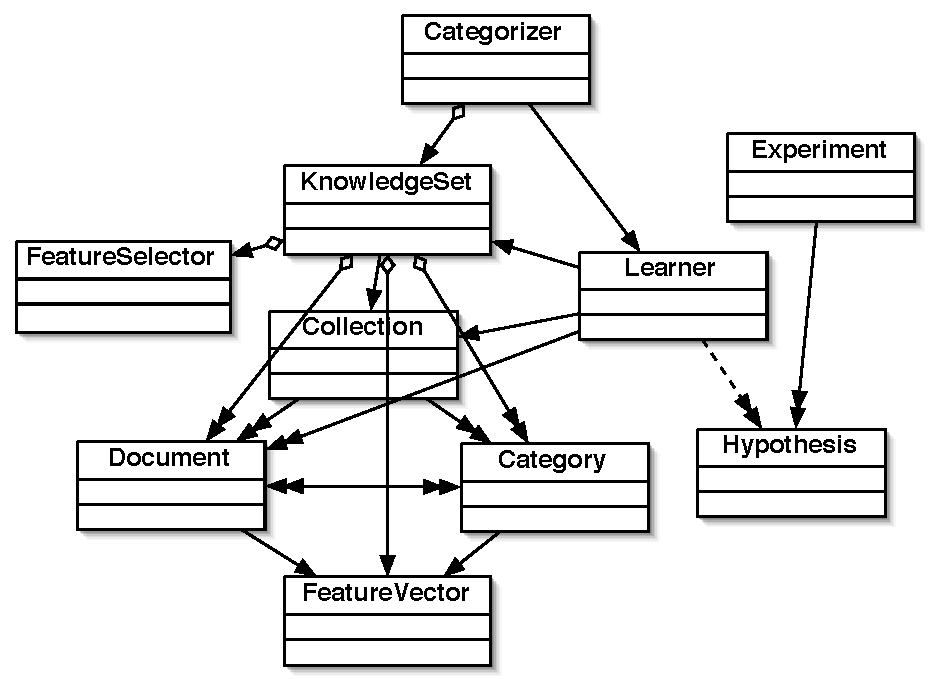
\includegraphics[width=\linewidth]{classes-uml.pdf}
\caption{Simplified UML class diagram for the framework}
\label{classes-uml}
\end{figure}

\subsection*{Data format}
Since documents come in a wide variety of formats such as XML, plain text,
or PDF, the framework should support the
importing of knowledge in several formats and have a mechanism by
which the user may extend these capabilities for a particular
environment.  The base class \texttt{Document} allows the user to
specify the content as a string.  The user may also subclass the
\texttt{Document} class, overriding the \texttt{parse()} method for
direct importing of data in its natively stored format.

In the \texttt{Collection} class and its subclasses, the framework
also supports the notion of a collection of stored documents, such as
a directory of text files, a database of stored documents, or an XML
file containing multiple documents.  The most common storage formats
can be a part of the core framework, while proprietary or unusual
formats can be implemented through subclassing.  Note that the
document format and collection format are independent characteristics;
a project may have a directory of text files, a directory of XML
files, or a directory of PDF files, but these would all be handled by
the \texttt{Collection::Files} class with the appropriate
\texttt{Document::} class.  Likewise, a project may have a collection
of XML documents stored in a single file, as a directory of files, or
in a database, but these would all be parsed by the
\texttt{Document::XML} class with the appropriate \texttt{Collection}
class. Note that \texttt{Document} and its subclasses exist mainly for
the purpose of importing data; after the data is read and parsed, the
rest of the system will throw away the \texttt{Document} object,
keeping only its \texttt{FeatureVector} object and the list of
\texttt{Categories} associated with the \texttt{Document}.

\subsection*{Structured documents}
Each document may have several sections of content, such as ``body'',
``subject'', ``signature'', and so on.  In \texttt{AI::Categorizer},
the user specifies the content by providing a hash of key-value pairs,
where the key indicates the name of the section, and the value is a
string containing the content data.  The user may also specify
``weights'' to assign to the features found in each section.  In the
future, other treatments for the different sections of a document may
be supported as we develop effective ways to use
this structure.


\subsection*{Tokenizing of data}
The default implementation tokenizes document data by extracting 
all non-whitespace byte sequences between word-character 
boundaries.  This is usually sufficient in English,
but non-English language documents or documents with unusual content
will certainly necessitate custom tokenization.  To achieve this, the
user may subclass the \texttt{Document} class and override its
\texttt{tokenize()} method if a different algorithm is required.  We
may also add other tokenizing options to the default implementation,
controlled by parameters, if other common tokenizing needs are found.

\subsection*{Linguistic stemming}
The default implementation provides support for the Porter stemming
algorithm, a standard algorithm for removing morphemes from English
words to obtain their ``stems,'' or root forms.  By default no
stemming is performed, but a \texttt{stemming} parameter can be set to
\texttt{porter} to activate stemming.  Alternatively, the user may
override the \texttt{stem\_words()} method of the \texttt{Document}
class for custom stemming.  This may be extremely important in highly
morphological languages or in certain application domains.

\subsection*{Feature selection}
Feature selection is handled by the \texttt{KnowledgeSet} class's
\texttt{scan\_features()} and \texttt{select\_features()} methods.
The \texttt{select\_features()} method works on an entire
\texttt{KnowledgeSet} in-memory at once.  The
\texttt{scan\_features()} method is a quicker and less
memory-consuming way to select features before reading in the whole
data set, but it requires the user to make two passes through the data
set to actually read in the documents.  Both methods return a
\texttt{FeatureVector} (feature vs. value) to the framework, which
saves the list of highest-ranking features to use when parsing future
documents.

The default implementation uses a simple Document-Frequency criterion
for selecting features to use in model-building and categorization.
This is very efficient, and has been shown in \cite{yang:97} to be
competitive with more elaborate criteria in many common situations.
We will add more criteria as the project develops.

\subsection*{Vector space modeling}
The full range of TF/IDF weighting from \cite{salton:88} are
supported, controlled by a \texttt{tfidf\_weighting} parameter.  If
the user wants to employ a different weighting scheme, the
\texttt{weigh\_features()} method in the \texttt{KnowledgeSet} class
may be overridden.

\subsection*{Machine Learning algorithm}
Choosing machine learning algorithms is done
by choosing a subclass of the \texttt{Learner} class.  Several
algorithms have already been implemented including \naive\ Bayes
\cite{lewis:98}, Support Vector Machines \cite{scholkopf:99}
\cite{cortes:95}, Neural Networks \cite{calvo:01} \cite{yang:99},
k-Nearest Neighbors \cite{yang:99}, and Decision Trees
\cite{quinlan:89}.  Any \texttt{Learner} class needs to implement the
virtual methods \texttt{create\_model()} and \texttt{get\_scores()},
which supply the semantics behind the \texttt{train()} and
\texttt{categorize()} methods, respectively.  Since many Machine
Learning algorithms are implemented as a series of binary decisions
concerning individual category memberships, an abstract
\texttt{Learner::Boolean} class is provided to help developers of new
categorizers--in this case, one need only implement the smaller
\texttt{create\_boolean\_model()} and \texttt{get\_boolean\_score()}
methods.

Note that the \texttt{Learner} class does dual duty as a learner and a
categorizer.  No class distinction is made in the framework between a
\texttt{Learner} before and after it has been trained--they are
objects of the same class.  This allows for the possibility of on-line
learning, in which a trained learner incrementally uses additional
training examples to improve its current model.

\subsection*{Machine Learning parameters}
Because each ML algorithm may have several implementation parameters
to control behavior, each \texttt{Learner} subclass accepts different
parameters.  To facilitate the wide variety of parameters that
different classes may require, we use the \texttt{Class::Container}
module\footnote{available at http://search.cpan.org/author/\\
KWILLIAMS/Class-Container-0.08/}.  This module allows each
\texttt{Learner} subclass to declare the parameters it accepts, so
that a Neural Network class can declare arguments for number of input,
hidden, and output nodes, a k-Nearest Neighbor class can declare
arguments for $k$ and for thresholding strategies, and so on.  These
parameters are passed through the framework transparently using a
variation on the ``Factory Method'' pattern. \cite{gamma:95}

In fact, the \texttt{Learner} and its subclasses are not the only
pieces of the framework in which varying parameters control
operations.  Because this situation is common throughout the
framework, \texttt{Class::Container} is employed consistently for all
structural classes in the framework.  This goes a long way toward
reducing the number of classes necessary to implement varying
behavior.

\subsection*{Hypothesis behavior}
Certain applications (e.g. newswire categorizers) may need to find
``all categories that apply'' for each document, whereas other
applications (e.g. automatic email routers) may only be interested in
the ``best N categories,'' where N is often 1.  These scenarios are
supported by the Hypothesis class, which provides a generic interface
to the scoring decisions of the categorizers.  Methods like
\texttt{categories()}, \texttt{best\_category()}, and
\texttt{in\_category()} provide application-level access to
categorization decisions based on the scores assigned by the
\texttt{Learner} class.

\subsection*{On-line training}
Some machine learning algorithms can easily integrate new knowledge
into the knowledge base without going through the potentially
expensive process of re-training the categorizer from scratch.  For
instance, most kNN implementations can do this, whereas most Neural
Network implementations cannot.  For categorizers that support this, a
virtual \texttt{add\_knowledge()} method in the \texttt{Learner} class
is supplied.  Currently no \texttt{Learner} subclasses in
\texttt{AI::Categorizer} support on-line learning, but the
architecture supports it when an implementation is needed.


\section{Framework Customization}

Like C++ and Java, Perl is natively object-oriented, but unlike them it does not have strict separation of compilation and execution stages.  Rather, the compiler and interpreter work in tandem, trading back and forth to execute a Perl application, allowing runtime compilation of code.  In addition, Perl's object model is fairly loosely bound (similar in this respect to Objective-C's model), permitting class names to be stored in variables and/or specified at runtime.  Because of these properties, the choice of specific classes to be used in the framework can be made at runtime, controlled by parameters, facilitated by the \texttt{Class::Container} module.  It allows several classes to cooperate as a framework without having to know about each others' class names, constructor parameters, and so on, and provides the glue to do strict early checking of parameter names and types, facilitating transparent factory patterns within the framework.

For instance, to use the built-in SVM learner, one could either create
an \texttt{AI::Categorizer::SVM} object directly, or one could specify
the class name by providing it as a value for the
\texttt{learner\_class} parameter.  This behavior is implemented at
the framework level, so different \texttt{Document},
\texttt{Collection}, \texttt{FeatureVector}, etc. classes can be
pressed into service by the \texttt{document\_class},
\texttt{collection\_class}, and \texttt{feature\_vector\_class}
parameters, respectively.  This helps facilitate quick architectural
changes, letting developers drop their own subclasses into the
framework with relative ease.


\section{Evaluation}

Although the focus of this paper is the framework discussion and
design, we present here some basic evaluation of its performance.
We have evaluated our framework by building classifiers in several
applications.  We have implemented \naive\ Bayes, Support Vector
Machine, k-Nearest-Neighbor, and Decision Tree classifiers in the
framework.  We have trained classifiers using the standard Reuters
ApteMod corpus, and obtained similar results to the ones described in
\cite{yang:99}.  We have also trained and tested classifiers on other
corpora in financial, educational, and discussion group domains.  Due
to space constraints and the proprietary nature of some of our other
corpora, we will only describe results on the Reuters ApteMod corpus
here, using the \naive\ Bayes algorithm.

In training categorizers, we typically use two passes through the
corpus when loading the data.  The first pass scans the documents in
order to perform feature selection, while the second pass actually
loads the data into memory.  This allows memory to be used more
effectively than if we only made one pass over the data, because we
avoid loading extraneous features.  On the Reuters corpus, the first
pass over the 7769 training files may take roughly 59 CPU seconds and
consume 11 MB of memory, while the second pass takes about 57 CPU
seconds and consumes 32 MB\@.  The memory figures reflect the total
size of a running program, not just the size of the document data in
memory.\footnote{Tests were performed on a machine with a Pentium III
800Mhz chip, running Red Hat Linux release 7.0 and Perl 5.6.1.
Results are not comparable across different architectures, but may be
useful as a rough guide.}

After the data is loaded, we pass it to a Learner object for training.
Our \naive\ Bayes training process takes 8.1 CPU seconds and consumes
40 MB of memory.  Categorizing the 3019 test documents takes about 95
CPU seconds and consumes 14 MB.

With experimental settings similar to the ones described in
\cite{yang:99} (we used Document Frequency feature selection, since we
have not yet implemented $\chi^2$ or Information Gain selection
algorithms), we achieve recall, precision, and $F_1$ scores of 0.724,
0.851, and 0.782 when micro-averaged, and 0.366, 0.497, and 0.396 when
macro-averaged.  We believe any discrepancies with \cite{yang:99} are
due to differences in feature selection and/or document tokenizing,
but we have not tested this belief thoroughly.

\section{Integration and Further Work}


The framework has been used in a number of applications including an
extension to the SQL language of the PostgreSQL relational
database. It has also been used as distributed service for
classification using an XML/RPC architecture, and integrated into
multi-tier web applications and desktop applications.

We know that much work has been done by previous developers and
researchers in the area of Text Categorization.  While we are in one
sense re-treading ground by implementing generic TC software, we see
our work as a way to extend the reach of others' work, rather than as
a replacement for it.

To this end, we have tried to make the framework very inter-operable
and provide interfaces to existing TC products.  For instance, we have
implemented a \texttt{Learner} subclass called \texttt{Learner::Weka}
to provide an interface to any Weka classifier the user would like to
use.  In this way, \texttt{AI::Categorizer} benefits when progress is
made in Weka, as well as the other way around.

We hope to create interfaces to other existing products as well.  If the
\texttt{AI::Categorizer} project gains enough momentum that other
people wish to contribute code to it, we will encourage this code to
be as independent and generic as possible so that we may simply
create an interface to it in our framework.  For instance, this is 
how the SVM learner in our framework was created recently--our
\texttt{AI::Categorizer::SVM} class is just a thin wrapper around a
generic \texttt{Algorithm::SVM} module by another author we
collaborated with, and this in turn is a wrapper around the C library
\texttt{libsvm}.

It is our hope that this strategy will extend the reach of both our
framework and related existing and new TC software.

In designing the AI::Categorizer framework architecture, we have
focused on aspects of Text Categorization that tend to remain common
from one task to the next, allowing for growth in aspects that tend to
change.  For instance, we have specified that document features are
encapsulated in a FeatureVector object, but we have not specified that
object's internal implementation.  Likewise, we have specified that
the Machine Learning TC algorithms are encapsulated by the Learner
class, but the specific algorithms will tend to vary from task to
task.

In the first public versions of the framework, we have tended to
implement the simplest versions of each of these classes, with more
elaborate or optimized implementations deferred to later work.  For
instance, our FeatureVector class is currently implemented using Perl
hashes, but other implementations (for instance, using C structs to
implement sparse integer vectors) may be implemented in order to
improve memory usage and/or speed.  Other Learner subclasses may also
be added, and the existing subclasses may be improved to provide more
feature-rich implementations or improve efficiency.  Because they are
encapsulated in subclasses, these implementations may be traded at
will, allowing experimentation with different implementations.  In
particular, we expect the Learner and FeatureSelector areas of the
framework to grow as new algorithms are added and existing algorithms
are informed by current research.


\section{Conclusions}

We have developed a new framework for Text Categorization which is
publicly available and leverages existing work as much as possible.
We have primary goals of providing usable TC software for application
developers, researchers, and domain experts, as well as providing
bridges between existing and new TC software.  Our framework design
endeavors to embody the key requirements which are common to most work
in TC, and thus should improve reusability of design and
implementation in applications that use text categorization.  The
analysis of its architecture may be useful to those embarked in building
their own TC systems, so we have discussed the design decisions of the
different functionalities supported by the framework.

Periodic point-releases of \texttt{AI::Categorizer} are available at
http://www.cpan.org/modules/by-authors/id/KWILLIAMS/ , and
bleeding-edge development versions are available via CVS at
http://www.sourceforge.net/projects/ai-categorizer/ .


\bibliographystyle{sample}
\bibliography{TC-references}


\end{document}
